\documentclass[10pt,a4paper]{article}
\usepackage[utf8]{inputenc}
\usepackage[english]{babel}
\usepackage[activate={true,nocompatibility},final,tracking=true,kerning=true,spacing=true]{microtype}
\usepackage[plainpages=false,pdfpagelabels,unicode]{hyperref}
\usepackage{fullpage}
\usepackage{graphicx}
\usepackage{fancyhdr}
\usepackage{occi}
\setlength{\headheight}{13pt}
\pagestyle{fancy}

%  just a test
% default sans-serif
\renewcommand{\familydefault}{\sfdefault}

% no lines for headers and footers
\renewcommand{\headrulewidth}{0pt}
\renewcommand{\footrulewidth}{0pt}

% header
\fancyhf{}
\lhead{GFD-R}
\rhead{\today}

% footer
\lfoot{occi-wg@ogf.org}
\rfoot{\thepage}

% paragraphs need some space...
\setlength{\parindent}{0pt}
\setlength{\parskip}{1ex plus 0.5ex minus 0.2ex}

%\renewcommand\paragraph{%
%  \@startsection{paragraph}{4}{0mm}%
%     {-\baselineskip}%
%     {.5\baselineskip}%
%     {\normalfont\normalsize\bfseries}}

% some space between header and text...
\headsep 13pt

\setcounter{secnumdepth}{4}

\begin{document}

% header on first page is different
\thispagestyle{empty}

Draft \hfill  Thijs Metsch, Intel\\
OCCI-WG \hfill  Mohamed Mohamed, Telecom SudParis\\
\rightline {\today}

\vspace*{0.5in}

\begin{Large}
\textbf{Open Cloud Computing Interface -- Platform}
\end{Large}

\vspace*{0.5in}

\underline{Status of this Document}

\input{include/status}

\underline{Copyright Notice}

Copyright \copyright ~Open Grid Forum (2014-2015). All Rights
Reserved.

\underline{Trademarks}

OCCI is a trademark of the Open Grid Forum.

\underline{Abstract}

This document, part of a document series produced by the OCCI working
group within the Open Grid Forum (OGF), provides a high-level
definition of a Protocol and API. The document is based upon
previously gathered requirements and focuses on the scope of important
capabilities required to support modern service offerings.


\newpage
\tableofcontents
\newpage

\section{Introduction}
The Open Cloud Computing Interface (OCCI) is a RESTful Protocol and
API for all kinds of management tasks. OCCI was originally initiated
to create a remote management API for IaaS%
\footnote{Infrastructure as a Service}
model-based services, allowing for the development of interoperable tools for
common tasks including deployment, autonomic scaling and monitoring.
%
It has since evolved into a flexible API with a strong focus on
interoperability while still offering a high degree of extensibility. The
current release of the Open Cloud Computing Interface is suitable to serve many
other models in addition to IaaS, including PaaS and SaaS.

In order to be modular and extensible the current OCCI specification is
released as a suite of complimentary documents, which together form the complete
specification.
%
The documents are divided into four categories consisting of the OCCI Core,
the OCCI Protocols, the OCCI Renderings and the OCCI Extensions.
%
\begin{itemize}
\item The OCCI Core specification consists of a single document defining the
 OCCI Core Model. The OCCI Core Model can be interacted with through {\em
 renderings} (including associated behaviors) and expanded through {\em extensions}.
\item The OCCI Protocol specifications consist of multiple documents, each
 describing how the model can be interacted with over a particular protocol (e.g. HTTP, AMQP etc.).
 Multiple protocols can interact with the same instance of the OCCI Core Model.
\item The OCCI Rendering specifications consist of multiple documents, each
 describing a particular rendering of the OCCI Core Model. Multiple renderings can
 interact with the same instance of the OCCI Core Model and will automatically support
 any additions to the model which follow the extension rules defined in OCCI
 Core.
\item The OCCI Extension specifications consist of multiple documents,
  each describing a particular extension of the OCCI Core Model. The
  extension documents describe additions to the OCCI Core Model
  defined within the OCCI specification suite.
\end{itemize}
%

The current specification consists of seven documents. This
specification describes version 1.2 of OCCI and is backward compatible with 1.1.
Future releases of OCCI
may include additional protocol, rendering and extension specifications. The specifications to be
implemented (MUST, SHOULD, MAY) are detailed in the table below.

\mytablefloat{
	\label{tbl:occi_compliancy}%
	What OCCI specifications must be implemented for the specific version.
}
{
	\begin{tabular}{lll}
	\toprule
	Document & OCCI 1.1 & OCCI 1.2 \\
	\colrule
	Core Model & MUST & MUST \\
	Infrastructure Model  & SHOULD & SHOULD \\
	Platform Model & MAY & MAY \\
	SLA Model & MAY & MAY \\
	HTTP Protocol & MUST & MUST \\
	Text Rendering& MUST & MUST \\
	JSON Rendering& MAY & MUST \\
	\botrule
	\end{tabular}
}

% hello


OCCI makes an ideal interoperable boundary interface between the web
and the internal resource management system of platform providers.

\section{Notational Conventions}
\input{include/notational}

% begin platform content

\section{Platform}

The OCCI Platform document details how an OCCI implementation can model and implement a Platform as a Service API offering by extending the OCCI Core Model. This API enables the provisioning and management of PaaS resources. For example, it allows to deploy an application on one or more PaaS components. The application itself could be composed of different components. The main platform types defined within OCCI Platform are:

\begin{description}
  \item[Application] Which defines the user-defined part of the overall service.
  \item[Component] A configured instance of a piece of code providing business functions that are part of the execution of the application or responsible of hosting the application.
  \item[ComponentLink] Connects an \hl{Application} instance to a hosting \hl{Component} or connects two components.
\end{description}

\begin{figure}[!h]
	{\centering \resizebox*{0.7\columnwidth}{!}{\rotatebox{0}
	{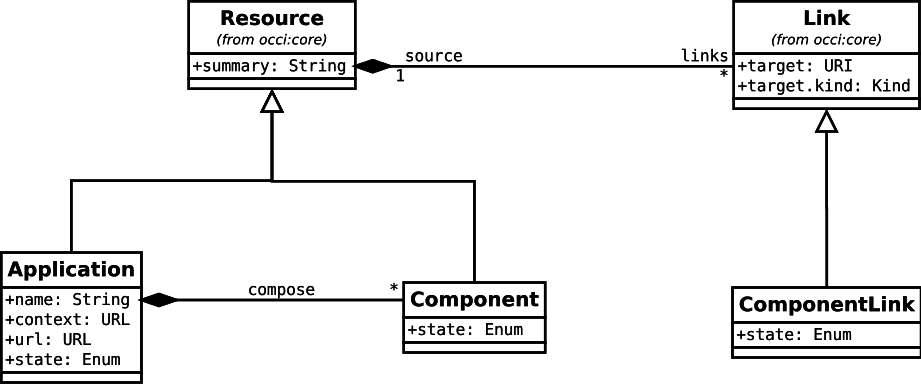
\includegraphics[scale=0.4]{figs/platform_overview.png}}} \par}
	\caption{Overview Diagram of OCCI Platform Types.}
	\label{fig:platform_uml}
\end{figure}

These platform types inherit the OCCI Core Model Resource base type and all their attributes. One can use a suitable transport protocol (e.g., HTTP) and a suitable rendering to discover and consume these resources. Independently of the implementation, the defined resources could be discoverable during runtime through OCCI compliant interfaces.

As required by the OCCI Core Model specification, every instantiated type that is a  sub-type of \hl{Resource} or \hl{Link} MUST be assigned a \hl{Kind} that identifies the instantiated type. Each such \hl{Kind} instance MUST be related to the Resource or Link base type's \hl{Kind}. That assigned \hl{Kind} instance MUST always remain immutable to any client.

\subsection{Application Kind Definition}
The following kind MUST be present and represents the kind definition of an application resource.

\hl{Application} inherits the \hl{Resource} base type defined in OCCI Core Model \cite{occi:core}. \hl{Application} is assigned the \hl{Kind} instance \textit{http://schemas.ogf.org/occi/platform\#application}. An \hl{Application} instance MUST use and expose this \hl{Kind}. The \hl{Kind} instance assigned to the \hl{Application} type MUST be related to the \textit{http://schemas.ogf.org/occi/core\#resource} \hl{Kind} by setting the \texttt{parent} attribute.

\mytablefloat{
	\label{tbl:app}\hl{Attribute}s defined for the \hl{Application} type.
}
{
	\begin{tabular}{lp{2.5cm}p{1cm}lp{5cm}}
	\toprule
	Attribute&Type&Multi\-plicity&Mutability&Description\\
	\colrule
	occi.app.name & String & 1 & Mutable & Name of the application.\\
	occi.app.context & URL & 1 & Immutable & URL for contextualizing the app.\\
	occi.app.url & URL & 1 & Immutable & DNS entry.\\
	occi.app.state & Enum \{active, inactive, error\} & 1 & Immutable & State of the application.\\
	occi.app.state.message & String & 0..1 & Immutable & Human-readable explanation of the current instance state.\\
	\botrule
	\end{tabular}
}

Table~\ref{tbl:app} describes the \hl{Attribute}s defined by an \hl{Application} instance. These attributes MAY or MUST be exposed by an instance of the \hl{Application} type depending on the ``Multiplicity'' column in the aforementioned table.

The \hl{Action}s are defined by the \hl{Kind} instance \textit{http://schemas.ogf.org/occi/platform\#application}. Every \hl{Action} instance in the table uses the \textit{http://schemas.ogf.org/occi/platform/application/action\#} categorisation scheme. ``Action Term'' below refers to \texttt{\hl{Action}.term}.

\mytablefloat{
	\label{tbl:app_actions}
	\hl{Action}s applicable to instances of the \hl{Application} type.
}
{
	\begin{tabular}{lll}
	\toprule
	Action Term & Target state & Attributes \\
	\colrule
	start & active & -- \\
	stop & inactive & -- \\
	\botrule
	\end{tabular}
}

The state model for the \hl{Application} instance is defined in Fig.~\ref{fig:app_state}.

\begin{figure}[!h]
	{\centering \resizebox*{0.5\columnwidth}{!}{\rotatebox{0}
	{\includegraphics[scale=0.2]{figs/platform_component_state.png}}} \par}
	\caption{State model of an \hl{Application} instance.}
	\label{fig:app_state}
\end{figure}

\subsection{Component Kind Definition}
The following kind MUST be present and represents the kind definition of a component resource.

\hl{Component} inherits the \hl{Resource} base type defined in OCCI Core Model \cite{occi:core}. \hl{Component} is assigned the \hl{Kind} instance \textit{http://schemas.ogf.org/occi/platform\#component}. A \hl{Component} instance MUST use and expose this \hl{Kind}. The \hl{Kind} instance assigned to the \hl{Component} type MUST be related to the \textit{http://schemas.ogf.org/occi/core\#resource} \hl{Kind} by setting the \texttt{parent} attribute.

\mytablefloat{
	\label{tbl:component}\hl{Attribute}s defined for the \hl{Component} type.
}
{
	\begin{tabular}{lp{2.5cm}p{1cm}lp{5cm}}
	\toprule
	Attribute&Type&Multi\-plicity&Mutability&Description\\
	\colrule
	occi.component.state & Enum \{active, inactive, error\} & 1 & Immutable & State of the component.\\
	occi.component.state.message & String & 0..1 & Immutable & Human-readable explanation of the current instance state.\\
	\botrule
	\end{tabular}
}

Table~\ref{tbl:component} describes the \hl{Attribute}s defined by \hl{Component} instance. These attributes MAY or MUST be exposed by an instance of the \hl{Component} type depending on the ``Multiplicity'' column in the aforementioned table.

The \hl{Action}s are defined by the \hl{Kind} instance \textit{http://schemas.ogf.org/occi/platform\#component}. Every \hl{Action} instance in the table uses the \textit{http://schemas.ogf.org/occi/platform/component/action\#} categorisation scheme. ``Action Term'' below refers to \hl{Action}.{\tt term}

\mytablefloat{
	\label{tbl:component_actions}
	\hl{Action}s applicable to instances of the \hl{Application} type.
}
{
	\begin{tabular}{lll}
	\toprule
	Action Term & Target state & Attributes \\
	\colrule
	start & active & -- \\
	stop & inactive & -- \\
	\botrule
	\end{tabular}
}

The state model for the \hl{Component} instance is defined in Fig.~\ref{fig:component_state}.

\begin{figure}[!h]
	{\centering \resizebox*{0.5\columnwidth}{!}{\rotatebox{0}
	{\includegraphics[scale=0.2]{figs/platform_component_state.png}}} \par}
	\caption{State model of a \hl{Component} instance.}
	\label{fig:component_state}
\end{figure}

\subsection{Linking to Components}

The composition of a service is realized through the linkage 
of \hl{Application} and \hl{Component} instances with each 
other. \hl{Application} can be linked to many \hl{Component} 
instances. This allows \hl{Application} and \hl{Component}s 
to form acyclic graphs. To illustrate this with an example, the 
\hl{Application} is the frontend, perceived by the user, to a 
composition of \hl{Component}s. To have a composition 
of \hl{Component}s (e.g. microservices) those \hl{Components} 
need to be related to one another (e.g. Applciation linking to 
its DB or the DB linking to a monitoring service). 

\hl{ComponentLink} inherits the \hl{Link} base type defined in OCCI Core Model \cite{occi:core}. \hl{ComponentLink} is assigned the \hl{Kind} instance \textit{http://schemas.ogf.org/occi/platform\#componentlink}. The \hl{Kind} instance assigned to the \hl{ComponentLink} type MUST be related to the \textit{http://schemas.ogf.org/occi/core\#link} \hl{Kind} by setting the \texttt{parent} attribute.

The \hl{ComponentLink} kind can be further enhanced by the use of  provider-specific Mixins. This can be used to expose details such as database access URIs for an application linked up with a database component.

\subsection{Platform Templates}
Platform Templates allow for clients of an OCCI implementation to quickly and conveniently apply predefined configurations to OCCI Platform defined types. They are implemented using Mixin instances. There are two supported platform template types in OCCI Platform.

\subsubsection{Application Template}
Application templates allow clients to define which underlying framework the application should use (e.g., Programming language).

The Application Template is defined by a Mixin. A provider-specific defined Application Template Mixin MUST relate to the OCCI Application Template Mixin through the \texttt{depends} attribute in order to give absolute type information. The OCCI Application Template is defined by the \textit{http://schemas.ogf.org/occi/platform\#app\_tpl} Mixin and MUST be supported should Application Templates be offered.

Provider-specific Application Templates are constructed using a ``term'' and ``scheme'' combination where the ``term'' is a provider-specific description of the framework (e.g., python, ruby, \dots{}). Where an implementation requires additional information to be held in the Templates Mixin, it MAY do so by using \hl{Category}’s inherited \hl{Attribute}s.

\subsubsection{Resource Template}
The Resource Template Mixin builds upon the concept of Application Templates. A Resource Template is a provider defined Mixin instance that refers to a preset Resource configuration.

This can be used to define the resource instance attributes of the application and component. The provider-specific Resource Templates are defined by using a ``term'' and ``scheme'' combination. Those provider-specific Resource Template Mixin must relate to the OCCI Resource Template defined by \textit{http://schemas.ogf.org/occi/} \textit{platform\#res\_tpl} through the \texttt{depends} attribute. Where an implementation requires additional information to be held in the Templates Mixin, it MAY do so by using \hl{Category}'s inherited \hl{Attribute}s.

An example of these templates is shown in the following UML diagram in Figure~\ref{fig:templates}.

\begin{figure}[!h]
	{\centering \resizebox*{0.7\columnwidth}{!}{\rotatebox{0}
	{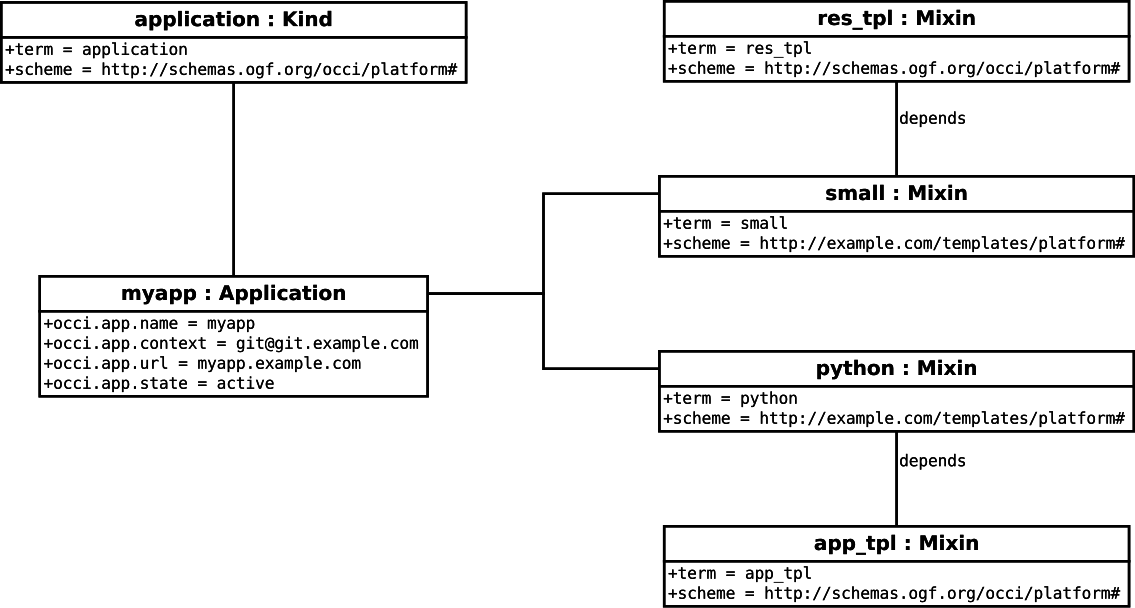
\includegraphics[scale=0.5]{figs/platform_templates.png}}} \par}
	\caption{Application and Resource Templates.}
	\label{fig:templates}
\end{figure}

\section{Specific Component Instance Mixins}
The following sections describe \hl{Mixin} instances, which SHOULD be implemented by Providers for some basic component type.

\subsection{Database Mixin}

\hl{Database} inherits the \hl{Mixin} base type defined in OCCI Core Model \cite{occi:core}. \hl{Database} is assigned the \hl{Mixin} instance \textit{http://schemas.ogf.org/occi/platform\#database}. The \hl{Database} instance \texttt{applies} to the \hl{Component} instance defined above.

\mytablefloat{
	\label{tbl:database}\hl{Attribute}s defined for the \hl{Database} type.
}
{
	\begin{tabular}{lp{2.5cm}p{1cm}lp{5cm}}
	\toprule
	Attribute&Type&Multi\-plicity&Mutability&Description\\
	\colrule
	occi.database.version & String & 1 & Immutable & Version of the database.\\
	\botrule
	\end{tabular}
}

Table~\ref{tbl:database} describes the \hl{Attribute}s defined by \hl{Database} instance.

\subsubsection{Database Link}
In case that an \hl{Application} instance links to a \hl{Component} instance, which has the \hl{Database} \hl{Mixin} instance applied the following \hl{Mixin} SHOULD be applied to the \hl{ComponentLink}.

\hl{DatabaseLink} inherits the \hl{Mixin} base type defined in OCCI Core Model \cite{occi:core}. \hl{DatabaseLink} is assigned the \hl{Mixin} instance \textit{http://schemas.ogf.org/occi/platform\#databaselink}. The \hl{DatabaseLink} instance \texttt{applies} to the \hl{ComponentLink} instance defined above.

\mytablefloat{
	\label{tbl:database_link}\hl{Attribute}s defined for the \hl{Database} type.
}
{
	\begin{tabular}{lp{2.5cm}p{1cm}lp{5cm}}
	\toprule
	Attribute&Type&Multi\-plicity&Mutability&Description\\
	\colrule
	occi.database.uri & URI & 1 & Immutable & Connection URI for the database instance.\\
	occi.database.username & URI & 0\ldots1 & Immutable & Username.\\
	occi.database.token & URI & 0\ldots1 & Immutable & Token.\\
	\botrule
	\end{tabular}
}

Table~\ref{tbl:database_link} describes the \hl{Attribute}s defined by \hl{DatabaseLink} instance.

% end platform content

\section{Security Considerations}
The OCCI Platform specification is an extension to the OCCI Core
Model specification \cite{occi:core}; thus the same security
considerations as for the OCCI Core Model specification apply
here.

\section{Glossary}
\label{sec:glossary}
\todo{update glossary}

\begin{tabular}{l|p{12cm}}
Term & Description \\
\hline
\hl{Action} & An OCCI base type. Represents an invocable operation on a \hl{Entity} sub-type instance or collection thereof. \\

\hl{Attribute} & A type in the OCCI Core Model. Describes the name and properties of attributes found in \hl{Entity} types. \\

\hl{Category} & A type in the OCCI Core Model and the basis of the OCCI type identification mechanism. The parent type of \hl{Kind}. \\

capabilities & In the context of \hl{Entity} sub-types {\bf  capabilities} refer
  to the OCCI \hl{Attribute}s and OCCI \hl{Action}s exposed by an {\bf entity
  instance}. \\

\hl{Client} & An OCCI client.\\

\hl{Collection} & A set of \hl{Entity} sub-type instances all associated to a particular \hl{Kind} or \hl{Mixin} instance. \\

\hl{Entity} & An OCCI base type. The parent type of \hl{Resource} and \hl{Link}. \\

entity instance & An instance of a sub-type of \hl{Entity} but not an instance
  of the \hl{Entity} type itself.  The OCCI model defines two sub-types of
  \hl{Entity}, the \hl{Resource} type and the \hl{Link} type.  However, the
  term {\em entity instance} is defined to include any instance of a
  sub-type of \hl{Resource} or \hl{Link} as well. \\

\hl{Kind} & A type in the OCCI Core Model. A core component of the OCCI classification system. \\

\hl{Link} & An OCCI base type. A \hl{Link} instance associates one \hl{Resource} instance with another. \\

\hl{Mixin} & A type in the OCCI Core Model. A core component of the OCCI classification system. \\

mix-in & An instance of the \hl{Mixin} type associated with an {\em entity
 instance}. The ``mix-in'' concept as used by OCCI {\em only} applies to
 instances, never to \hl{Entity} types. \\

model attribute & An internal attribute of a the Core Model which is {\em not}
  client discoverable. \\

\hl{OCCI} & Open Cloud Computing Interface. \\

OCCI base type & One of \hl{Entity}, \hl{Resource}, \hl{Link} or \hl{Action}. \\

OCCI Action & see \hl{Action}. \\
OCCI Attribute & A client discoverable attribute identified by an instance of the \hl{Attribute} type. Examples are \hl{occi.core.title} and \hl{occi.core.summary}. \\
OCCI Category & see \hl{Category}. \\
OCCI Entity & see \hl{Entity}. \\
OCCI Kind & see \hl{Kind}. \\
OCCI Link & see \hl{Link}. \\
OCCI Mixin & see \hl{Mixin}. \\

OGF & Open Grid Forum. \\

\hl{Resource} & An OCCI base type. The parent type for all domain-specific \hl{Resource} sub-types. \\

resource instance & See {\em entity instance}. This term is considered obsolete. \\

tag & A \hl{Mixin} instance with no attributes or actions defined. \\

template & A \hl{Mixin} instance which if associated at instance
creation-time pre-populate certain attributes. \\

type & One of the types defined by the OCCI Core Model.  The Core Model types are
 \hl{Category}, \hl{Attribute},
 \hl{Kind}, \hl{Mixin}, \hl{Action}, \hl{Entity}, \hl{Resource}
 and \hl{Link}. \\

concrete type/sub-type & A concrete type/sub-type is a type that can be instantiated.\\

URI & Uniform Resource Identifier. \\
URL & Uniform Resource Locator. \\
URN & Uniform Resource Name. \\
\end{tabular}


\section{Contributors}
We would like to thank the following people who contributed to this
document:

\begin{tabular}{l|p{2in}|p{2in}}
Name & Affiliation & Contact \\
\hline
Andy Edmonds & ICCLab, ZHAW & edmo at zhaw.ch \\
Peter Troeger & TU Chemnitz & peter@troeger.eu \\
Thijs Metsch & Intel & thijs.metsch@intel.com\\
Sami Yangui & & \\
Mohamed Mohamed & Telecom SudParis & \\
Philippe Merle & Inria & philippe.merle@inria.fr \\
\end{tabular}

Next to these individual contributions we value the contributions from
the OCCI working group.

\section{Intellectual Property Statement}
\input{include/ip}

\section{Disclaimer}
This document and the information contained herein is provided on an
``As Is'' basis and the OGF disclaims all warranties, express or
implied, including but not limited to any warranty that the use of the
information herein will not infringe any rights or any implied
warranties of merchantability or fitness for a particular purpose.


\section{Full Copyright Notice}
Copyright \copyright ~Open Grid Forum (2009-2016). All Rights Reserved.

This document and translations of it may be copied and furnished to
others, and derivative works that comment on or otherwise explain it
or assist in its implementation may be prepared, copied, published and 
distributed, in whole or in part, without restriction of any kind,
provided that the above copyright notice and this paragraph are
included as references to the derived portions on all such copies
and derivative works. The published OGF document from which such works
are derived, however, may not be modified in any way, such as by removing
the copyright notice or references to the OGF or other organizations,
except as needed for the purpose of developing new or updated OGF documents
in conformance with the procedures defined in the OGF Document Process,
or as required to translate it into languages other than English. OGF,
with the approval of its board, may remove this restriction for inclusion
of OGF document content for the purpose of producing standards in cooperation
with other international standards bodies. 

The limited permissions granted above are perpetual and will not be
revoked by the OGF or its successors or assignees.


\bibliographystyle{IEEEtran}
\bibliography{references}

\end{document}
